\documentclass[tikz,border=10pt]{standalone}
\usetikzlibrary{positioning, shapes.geometric, arrows.meta, calc}

\begin{document}

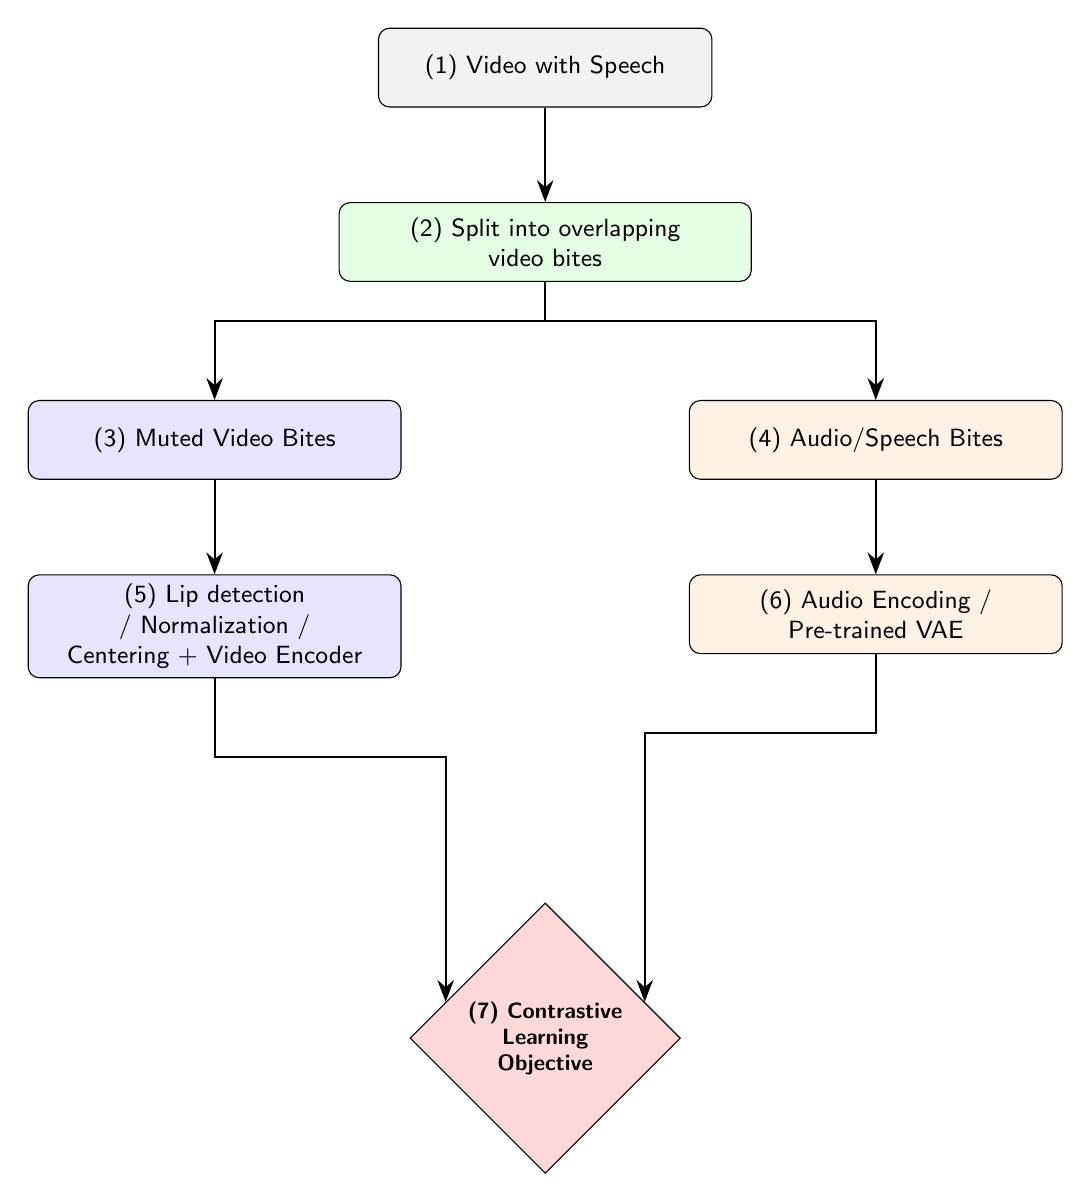
\begin{tikzpicture}[
    node distance=1.2cm and 1.5cm,
    % Define styles
    base/.style={rectangle, draw, align=center, minimum height=1cm, font=\sffamily\small, rounded corners},
    input/.style={base, fill=gray!10, text width=4cm},
    split/.style={base, fill=green!10, text width=5cm},
    branch/.style={base, fill=blue!10, text width=4.5cm},
    audio_branch/.style={base, fill=orange!10, text width=4.5cm},
    objective/.style={diamond, draw, fill=red!15, text width=2.5cm, align=center, font=\sffamily\bfseries\footnotesize, inner sep=0pt},
    arrow/.style={-{Stealth[scale=1.2]}, thick}
]

    % --- TOP LEVEL ---
    \node (raw_data) [input] {(1) Video with Speech};
    \node (split_bit) [split, below=of raw_data] {(2) Split into overlapping\\video bites};

    % --- THE SPLIT ---
    % We use the .south anchor of split_bit to start the branching
    \node (muted_video) [branch, below left=1.5cm and -0.8cm of split_bit] {(3) Muted Video Bites};
    \node (audio_bites) [audio_branch, below right=1.5cm and -0.8cm of split_bit] {(4) Audio/Speech Bites};

    % --- PROCESSING LAYER ---
    \node (video_proc) [branch, below=of muted_video] {(5) Lip detection / Normalization /\\Centering + Video Encoder};
    \node (audio_proc) [audio_branch, below=of audio_bites] {(6) Audio Encoding /\\Pre-trained VAE};

    % --- OBJECTIVE ---
    % Calculate the midpoint between the two bottom centers for the final loss diamond
    \node (cl_loss) [objective, below=3cm of $(video_proc.south)!0.5!(audio_proc.south)$] {(7) Contrastive\\Learning\\Objective};

    % --- DRAW CONNECTIONS ---
    \draw [arrow] (raw_data) -- (split_bit);
    
    % Branching arrows using south anchor and orthogonal paths
    \draw [arrow] (split_bit.south) -- ++(0,-0.5) -| (muted_video.north);
    \draw [arrow] (split_bit.south) -- ++(0,-0.5) -| (audio_bites.north);

    \draw [arrow] (muted_video) -- (video_proc);
    \draw [arrow] (audio_bites) -- (audio_proc);

    % Merging to Objective with right-angle bends
    \draw [arrow] (video_proc.south) -- ++(0,-1.0) -| (cl_loss.160);
    \draw [arrow] (audio_proc.south) -- ++(0,-1.0) -| (cl_loss.20);

\end{tikzpicture}

\end{document}